\documentclass[conference]{IEEEtran}
\IEEEoverridecommandlockouts
% The preceding line is only needed to identify funding in the first footnote. If that is unneeded, please comment it out.
%Template version as of 6/27/2024

% \usepackage{cite}
\usepackage{amsmath,amssymb,amsfonts}
\usepackage{algorithmic}
\usepackage{graphicx}
% Graphic path
% \graphicspath{{./pics/}}
\usepackage{textcomp}
\usepackage{xcolor}
\usepackage{orcidlink}
\usepackage{hyperref}
\usepackage{multirow}
\usepackage{float}
\usepackage{tikz}
\usetikzlibrary{positioning}
\usepackage{textcomp}
\usepackage{listings}
\usepackage{subcaption}

\lstset{
    basicstyle=\ttfamily,
    breaklines=true,
    breakatwhitespace=true,
    keepspaces=true,
    columns=fullflexible,
    showstringspaces=false,
    % Prevent word splitting
    % breakwords=true,
    % allowbreak=true,
    % postbreak=\mbox{\textcolor{red}{↪}},
    % Optional: prevent hyphenation
    % hyphenation=true
}

\def\BibTeX{{\rm B\kern-.05em{\sc i\kern-.025em b}\kern-.08em
    T\kern-.1667em\lower.7ex\hbox{E}\kern-.125emX}}
    
% \usepackage[
% backend=biber,
% style=IEEEtran,
% sorting=ynt
% ]{biblatex}
% \addbibresource{ref.bib}
\begin{document}


\title{The Eternal Adversary between Censor and Circumvention}
\footnotesize
% \textsuperscript{*}Note: Sub-titles are not captured for https://ieeexplore.ieee.org  and should not be used
%\thanks{Identify applicable funding agency here. If none, %delete this.}  

\author{\IEEEauthorblockN{1\textsuperscript{st} Guanru Chen}
\IEEEauthorblockA{\textit{Technische Universität München} \\
\textit{guanru.chen@tum.de \orcidlink{0009-0004-0715-910X}}}}
\maketitle

\begin{abstract}
This paper reviews and discussion the adversary between censorship and approaches to circumvent those restrictions from technical perspective. This paper discusses the current technologies in Aspect of Detection, Restriction, and Circumvention. We also actively collect, process, and visualize proxy traffic for obtaining supporting resources. We elaborate on the adversary on both sides, censor and circumvention and the current mainstream technologies about that.
\end{abstract}

\begin{IEEEkeywords}
Censorship, Firewall, Proxy, Encryption, TLS
\end{IEEEkeywords}

\section{Introduction}
Restrictions of network connectivity are everywhere and are deployed for various reasons: companies use such technologies for security audits and the prevention of commercial secrets leakages, parents use them to control children's screen time, and regimes also deploy them on a large scale to stifle freedom of thought… However, there are some approaches that try to circumvent it. In this article, we discuss the adversity between the rivals by focusing on technologies and their evolution from a technical perspective. 
The primary idea of restriction is simple: as an Internet service provider (ISP), censors can drop a packet with specific criteria (such as destination IP, destination port, protocol in TCP/IP 5 tuple). 
The primary idea of a proxy is also simple: through an external server as a relay (or springboard) to reach the site blocked by the local network.

\section{Related Work}
There are some existing works that discuss those technologies in specified aspects, such as TLS fingerprinting\cite{TLS_Fingerprinting}, active probing \cite{Active_Probing}, and analysis (or audition) of protocols \cite{shadowsocks_analysis} \cite{Trojan-Probe}. In this article, we intend to give an overview of these technologies with practical examples and real-world scenarios.

\section{Methodology}
We analyze typical protocols statically in our cloud servers and visualize the data.

\subsection{Protocols that We Took Into Consideration}
We chose typical protocols with different ideas:
\begin{enumerate}
    \item \href{https://shadowsocks.org}{Shadowsocks} (to be more specific, we use its newest rust-based implementation since it is still under active maintenance) and \href{https://gitlab.com/yawning/obfs4}{obfs4 bridge}, which represents the idea of encrypting and obfuscating.
    \item \href{https://trojan-gfw.github.io/trojan/}{trojan-gfw} and \href{https://github.com/klzgrad/naiveproxy}{naiveproxy}, which are practices of the concept to camouflage HTTPS connection and to utilize TLS for security.
    \item Plain HTTPS connection as a control group.
\end{enumerate}

\subsection{Set Up Proxy Server}
We configure the remote proxy server and the corresponding dependencies since most server sides of the TLS-based protocols require an upstream Web Server to forward unauthorized web traffic, which is always considered an active probe. For more details about how it can be utilised by censor in practice, please refer to section \ref{sec:active_detection}.
To make a TLS-based proxy server work, we must configure the proxy server program, the underlying "fallback" web server, and obtain a SSL certificate. For more about the mechanisms to combat active probing, especially the idea of "fallback", please refer to section \ref{sec:apc}. You can also find the sample configuration file in your repository. %See \ref{sec:config}.
% We publish the notes and more technical details about the servers' configuration processes in the seminar repository. 

\subsection{Data Collection by Capturing}
We use tcpdump \cite{tcpdump} to capture network traffic that flows through. 

\begin{lstlisting}[language=bash]
    tcpdump -G <capture interval> -W 1 -w <protocol name>.pcap -i <network interface> -n dst host <ip> and dst port <port> and <transmission protocol> --print
\end{lstlisting}

Specifying the enclosed parameters accordingly provides flexibility to filter traffic and interact with it.

\subsection{Processing and Analysis}
We implement a simple Python script with an external library, dpkt\cite{dpkt}, which spares the time and work to decode recorded pcap files and strip negligible packet headers of corresponding lower OSI layers (we should focus on proxy traffic). 
In the analysis phase, we select two aspects (the most remarkable characteristics of encrypted protocols): entropy and packet length. Additionally, we should consider and measure their variations in the temporal domain. 
For TLS-based protocols, their TLS fingerprints introduce a new characteristic. The concept of TLS fingerprint is a combination of various factors according to the standard of SSL/TLS, key exchange algorithm, asymmetric encryption algorithm, symmetric encryption algorithm, MAC algorithm, SSL version, and further derived experimental features, e.g. session resumption, multiplex/HTTP2). 
Sorting and evaluating such versatile, statistically relevant data requires further consideration. However, we still implement some auxiliary functions to retrieve cipher suite information from client hello (if no encryption is applied). 
We have made the code available in the seminar repository.

\section{The Censor}
Almost all firewalls try to restrict only specific traffic, with interference in authorized connections as little as possible, so there is a need for mechanisms to distinguish between valid and invalid connection attempts. 

\subsection{The detection}\label{sec:detection}
Generally speaking, two kinds of approaches try to achieve this goal: passive tests, which try to analyze the existing data and figure out characteristics and patterns that make a disguised traffic identifiable, and active probes, which use measurements such as replay attack, tampering data, and man-in-the-middle attack. We discuss different approaches that try to distinguish "unauthorized" traffic.

\subsection{The Passive Detection}
Passive detection means that the censor analyzes the traffic that goes through their infrastructures (the "Infrastructures" are often gateways but should not be limited to gateways, for example, they can also use optical splitters to intercept traffic from fibers). When people use network tools such as tcpdump or CharlesProxy\texttrademark{} to check traffic, they do almost the same work with the censor, but beyond the idea, the tools that are adopted by censors can sometimes be much more sophisticated. Traffic can be inspected in multiple OSI Layers. Also, different Protocols can be analyzed with different measurements depending on their characteristics (for example, we can analyze a HTTPS traffic with the help of a MITM Attack).

\subsubsection{Effort in decryption}
 The most straightforward way to decide whether a connection is valid is to retrieve the carried payload and censor it. But in the age of AEAD (authenticated encryption with associated data) and HTTPS/SSL, it becomes complicated or can only be partially implemented in a very stringent condition like an attack that utilizes a classical vulnerability Heartbleed \cite{Heartbleed}. In most scenarios, it has been patched. 
 \begin{itemize}
    \item  For symmetric-key algorithms, some extremely old encryptions before the advanced encryption standard (AES), such as single DES and RC-4 can be solved in a reasonable time. However, that is not a feasible approach because nowadays, most protocols (both TLS and non-TLS-based) have widely adopted AES algorithms.
    \item There can be more chances when considering the asymmetric-key exchange phases, which only happen when a TLS-based protocol tries to establish. For example, MITM attack, for more detail about MITM, please refer to section \ref{sec:mitm}, which goes on “Active Probing” since it needs to intercept and tamper packets. Shor’s algorithm \cite{Shors_Algorithm} also provides a possibility to solve the question in polynomial time. Still, due to versatile technical limitations, it is generally not practical (such an existing quantum computer’s capability is like "it could tell you there is 70\% chance 15 = $3\times$5").
 \end{itemize}


\subsubsection{Entropy}
Entropy is a remarkable factor in detecting a protocol, but it could not be the single factor since almost all ciphertexts have a high entropy. But it can be a factor together with the amount of traffic to make a preliminary decision whether a connection is suspicious and needs further investigation: high entropy (encrypted), long-lasting but non-HTTPS traffic can be an unauthorized attempt to connect, communicate, and transfer data between proxy client and proxy server. However the combination of those factors is not sufficient to determine it, or it introduces errors far beyond an acceptable range. 
We collect some of the typical encrypted protocols' traffic (both proxy protocols and genuine HTTPS protocol) and calculate its general entropy.
Here is the overall entropy of each proxy protocol
%we also verified our result with ent \cite{ent}.

\begin{table}[h]
\centering
\caption{Average Entropy for Common Protocols}
\resizebox{\columnwidth}{!}{
\begin{tabular}{|l|lllll|}
\hline
\multirow{2}{*}{} & \multicolumn{5}{c|}{Protocol Name}                                                                                                   \\ \cline{2-6} 
                  & \multicolumn{1}{l|}{Shadowsocks} & \multicolumn{1}{l|}{HTTPS} & \multicolumn{1}{l|}{NaiveProxy} & \multicolumn{1}{l|}{Trojan} & Obfs4 \\ \hline
Entropy          & \multicolumn{1}{l|}{7.999}      & \multicolumn{1}{l|}{7.977} & \multicolumn{1}{l|}{7.992}      & \multicolumn{1}{l|}{7.858}  & 7.999 \\ \hline
\end{tabular}%
}
\end{table}

% Current Revisiting Process

\subsubsection{TLS fingerprinting}
For a TLS-based protocol, it additionally exposes fingerprints, that are mainly about offered and chosen cipher suits(key exchange, MAC, Key Length…). There have been many protocols that try to camouflage HTTPS connections by design. 
The HTTPS (to be more specific, TLS, Transport Layer Security on which HTTPS is built) protocol stack brings extra advantage in the prospect of security since it is designed and verified rigorously in terms of cryptography. For example, with TLS's implementation, developers can be exempt from worrying about protecting the server from reply attacks. Without security features provided by TLS, they must build a Bloom Filter on their own. But a Bloom Filter can also be a suspicious characteristic.
On the other hand, a failed try to camouflage HTTPS traffic can be one of the most "deadly" remarkable characteristics \cite{TLS_Fingerprinting}. Except for the ciphers, there are many more factors that can be measured as fingerprints of HTTPS connections, which are initialized by a client, such as SSL/TLS version, certificates, multiplex (for HTTP/2), and more experimental features such as early data, TCP fast open (TFO). Such fingerprints can be used in conjunction with other factors, such as the packet length. We will elaborate on it later in the section \ref{section:cam}. 
There was a widely used Shadowsocks’ fork, ShadowsocksR, which tried to imitate HTTPS with an artificial SSL handshake. But when confronting a relatively mature and well-designed censor technology, those camouflages turned out to be a fatal vulnerability: it did not establish a real SSL connection, just attempts to make a fake handshake and attach an artificial HTTPS header.

\subsubsection{Behavior}
Behavior is a generic factor that covers the reaction of both client and server in different scenarios: how do they communicate? Do they send heartbeat packets to keep living? What happens in handshake phase? How do they exchange control instruction? These factors allow almost all professional routers to filter connections with OpenVPN or Wireguard protocol. But we focus on proxies such as obfs4 and Shadowsocks because most of the VPNs, together with SSH Tunnels, are not designed to have abilities to bypass censors (We are not going to talk about and consider some modified versions of OpenVPN, which are advertised as capable for censor bypassing, because they are always proprietary and do not follow an open standard). There are also behaviors worth researching and discussing, such as how servers react to active probes, see section \ref{sec:active_detection} "The Active Detection".

\subsubsection{Packet length}
The length of packets that carry the payload, header, and instructions of the proxy protocol is also a significant feature of protocols. An example is Trojan-gfw, which utilizes the TLS protocol stack but does not resize its packets. This leads to some packets with outstanding extreme lengths. 
The following figures that we depict show the occurrences of length respectively for each protocol. 
There are also length statistics of standard HTTPS traffic, which can be the control group. Naiveproxy uses padding and packet resizing to mitigate recognizing and categorization in the aspect of packet length. 

% \begin{figure}[H]
%     \centering
%     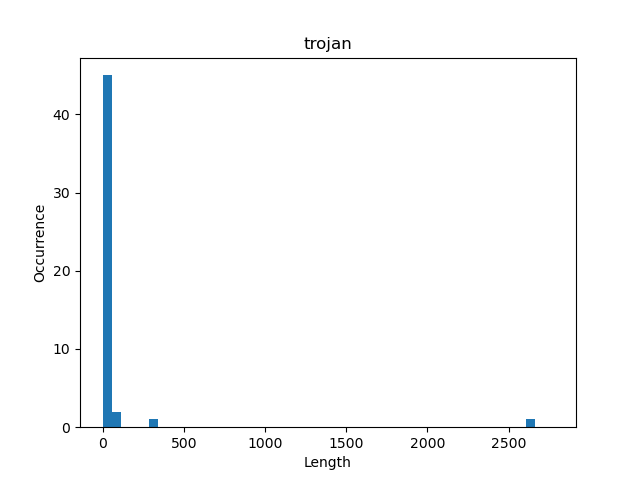
\includegraphics[width=0.4\textwidth, height=5cm]{pics/occurrence_of_length_trojan.png}
%     \caption{The length-occurrence statistics of Trojan-gfw}
% \end{figure}

% \begin{figure}[H]
%     \centering
%     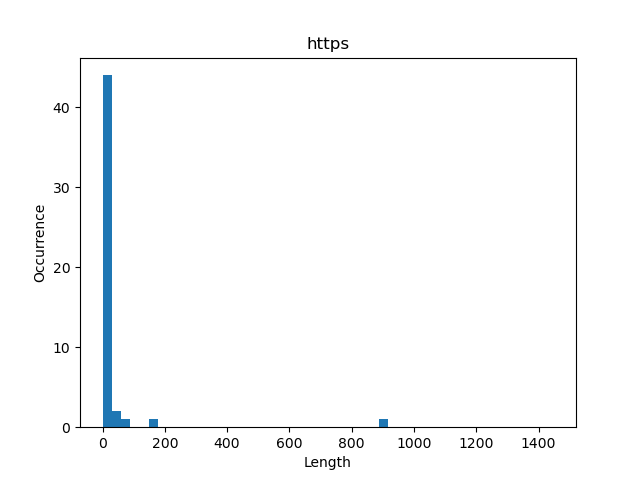
\includegraphics[width=0.4\textwidth, height=5cm]{pics/occurrence_of_length_https.png}
%     \caption{The length-occurrence statistics of HTTPS}
% \end{figure}

% \begin{figure}[H]
%     \centering
%     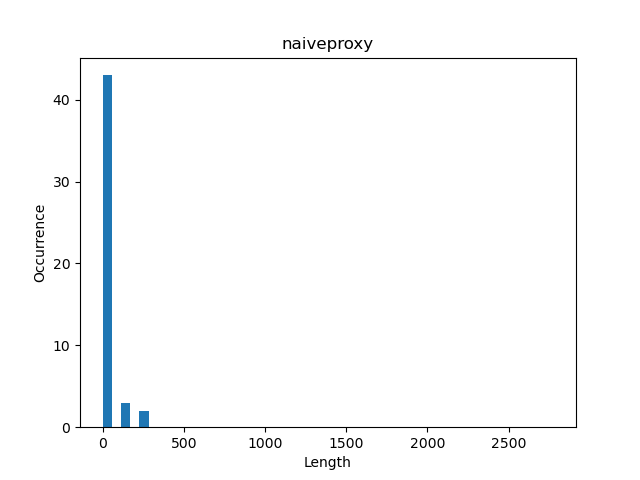
\includegraphics[width=0.4\textwidth, height=5cm]{pics/occurrence_of_length_naiveproxy.png}
%     \caption{The length-occurrence statistics of Naiveproxy}
% \end{figure}
\begin{figure}[H]
    \centering
    \begin{subfigure}[b]{0.40\textwidth}
        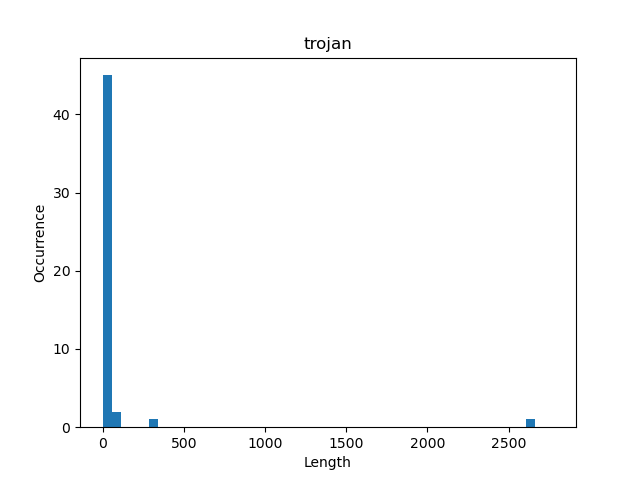
\includegraphics[width=\textwidth, height=4cm]{pics/occurrence_of_length_trojan.png}
        \caption{Trojan}
    \end{subfigure}
    \hfill
    \begin{subfigure}[b]{0.40\textwidth}
        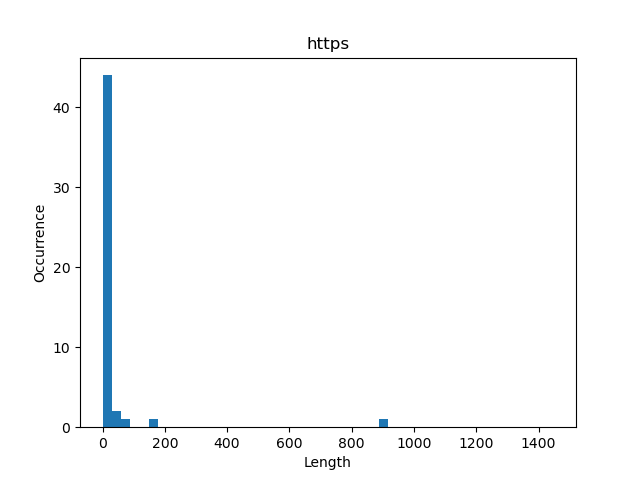
\includegraphics[width=\textwidth, height=4cm]{pics/occurrence_of_length_https.png}
        \caption{HTTPS}
    \end{subfigure}
    \hfill
    \begin{subfigure}[b]{0.40\textwidth}
        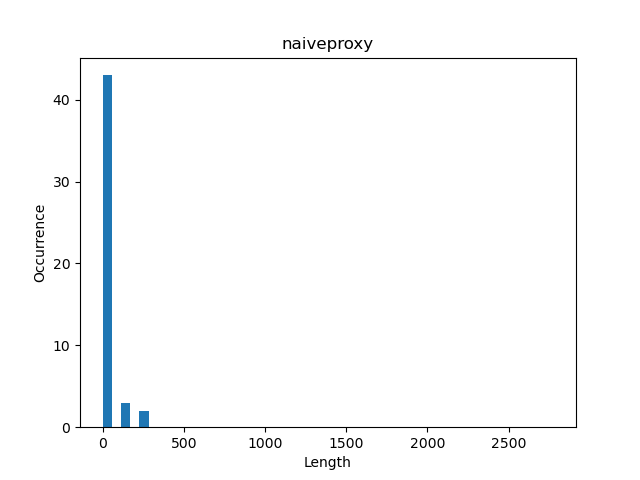
\includegraphics[width=\textwidth, height=4cm]{pics/occurrence_of_length_naiveproxy.png}
        \caption{Naiveproxy}
    \end{subfigure}
    \caption{Length-occurrence statistics}
\end{figure}

\subsubsection{Temporal domain (timing analysis)}
As a connection is a dynamic process, how traffic varies in the temporal domain is worth researching. The timing analysis shows its significance, especially when a remarkable process happens such as a handshake. 
We depict The variations of different protocols in the temporal domain. It is worth noticing that because of Shadowsocks' nature (they use preset symmetric private key), it does not need key exchange and handshake (the connection itself can be stateless)

\begin{figure}[H]
    \centering
    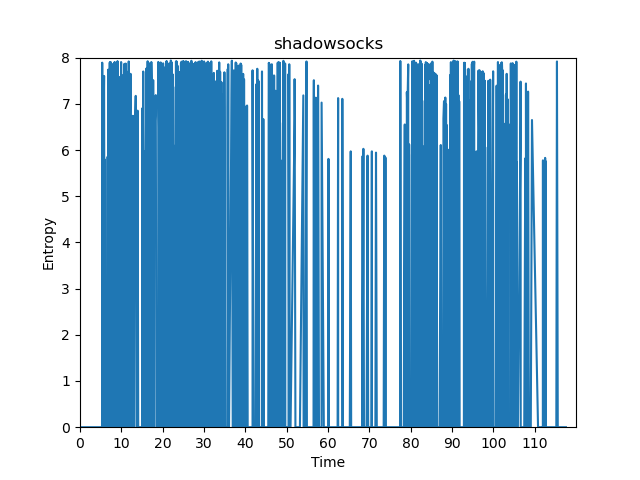
\includegraphics[width=0.40\textwidth, height=4cm]{pics/temporal_statistic_of_entropy_shadowsocks.png}
    \caption{The Entropy statistics of Shadowsocks in temporal domain}
\end{figure}

% \begin{figure}
%     \centering
%     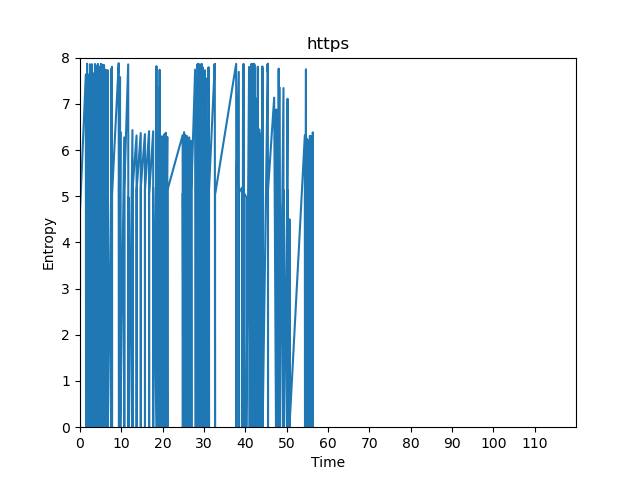
\includegraphics[width=0.45\textwidth]{temporal_statistic_of_entropy_https.png}
%     \caption{The Entropy Statistics of HTTPS in Temporal Domain}
%     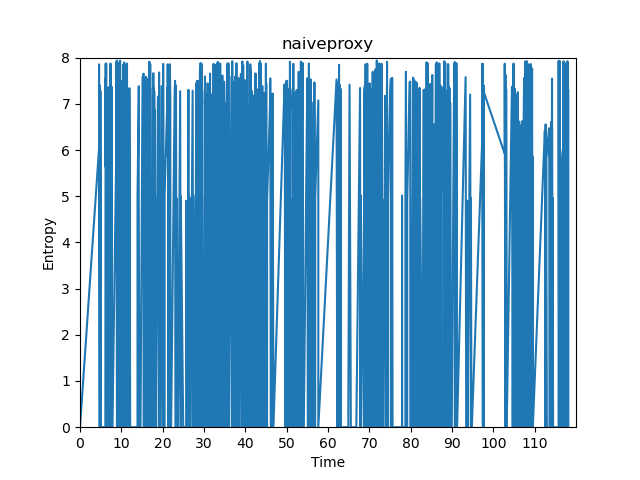
\includegraphics[width=0.45\textwidth]{temporal_statistic_of_entropy_naiveproxy.png}
%     \caption{The Entropy Statistics of Naiveproxy in Temporal Domain}
%     \centering
%     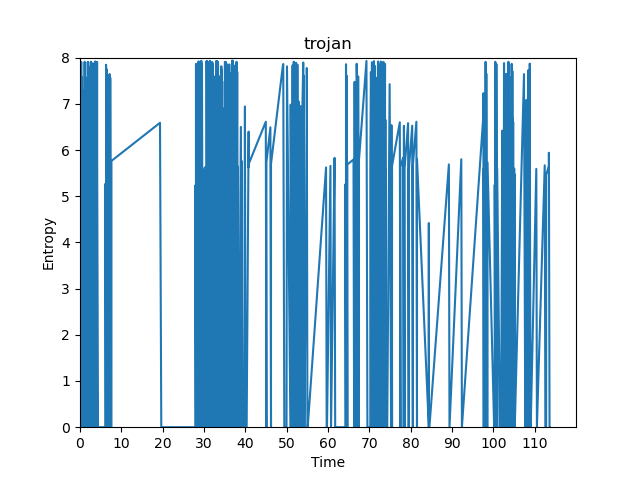
\includegraphics[width=0.45\textwidth]{temporal_statistic_of_entropy_trojan.png}
%     \caption{The Entropy Statistics of Trojan-gfw in Temporal Domain}
% \end{figure}

\subsubsection{Other miscellaneous factors}
There are also some miscellaneous outstanding characteristics, such as the structure of packets, special headers or bits (which is in even plaintext when a handshake happens). Classical VPNs and standard proxies that are not designed with the intention of providing censor bypass capability always have these characteristics. That's the reason most of industrial routers/gateways can distinguish and mark traffic as OpenVPN or Wireguard.

\subsection{The active detection}\label{sec:active_detection}
Active detection can be used as a supplement, but it is not so widely adopted as passive inspection (But in authoritarian countries that have an extreme network censor it is adopted), the main reason is scanning, probing, and sniffing are always regarded as "sensible" activities and associated with suspicious hack activities. But for national-level censors, who can control a large scale of malicious bot net. Because they have not only resources (of course, money from taxpayers) but also control the infrastructures of the backbone network.

\subsubsection{Man in the middle attack}\label{sec:mitm}
MITM attack is a common and practical way to decrypt TLS traffic due to the nature of asymmetric encryption: 
it is normal to practice MITM attacks in conjunction with downgrading attacks since network suppliers (for example ISPs, network administrators of enterprises or government) can always intercept, tamper, and mirror traffic which is carried by their links. 
Such attacks utilize the nature of the asymmetrical encryption and the key exchange process, which happens when a SSL/TLS channel tries to establish: the asymmetric encryption can guarantee the connection between peers is secure, but it cannot verify who the peer is. That means without further extra verification of the peer's identity (like a certificate issued by certificate authority CA), a man in the middle can easily fake the genuine peer and decrypt all the messages in your communication, as the following figure shows: through asymmetric encryption, there are two "secure" channels setup, but asymmetric encryption itself can not guarantee who the peer in another side of the "secure" channel is.

\begin{figure}[!h]
\centering
\usepackage{tikz}
\usetikzlibrary{positioning}
\begin{document}
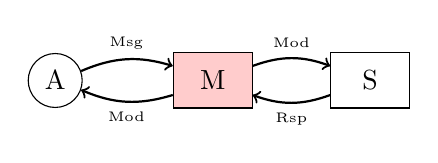
\begin{tikzpicture}[
    scale=0.4, % Further reduced scale
    node distance=2cm, % Further reduced distance
    user/.style={circle,draw,minimum size=0.6cm},
    attacker/.style={rectangle,draw,fill=red!20,minimum width=1cm,minimum height=0.7cm},
    server/.style={rectangle,draw,minimum width=1cm,minimum height=0.7cm}
]
    % Define nodes with shorter labels
    \node[user] (alice) {A};
    \node[attacker] (mitm) [right of=alice] {M};
    \node[server] (server) [right of=mitm] {S};

    % Shorter arrows and smaller labels
    \draw[->,thick] (alice) to[bend left=20] node[above,font=\tiny] {Msg} (mitm);
    \draw[->,thick] (mitm) to[bend left=20] node[above,font=\tiny] {Mod} (server);
    \draw[->,thick] (server) to[bend left=20] node[below,font=\tiny] {Rsp} (mitm);
    \draw[->,thick] (mitm) to[bend left=20] node[below,font=\tiny] {Mod} (alice);
\end{tikzpicture}
\end{document}
\caption{MITM attack: Attacker (M) intercepts messages between client (C) and server (S).}
\label{fig:mitm}
% \vspace{-0.2cm}
\end{figure}

Furthermore, they can even attack at the level of certification suites, such as coercing all the devices that are allowed to access their local network install and trust their own root certificate. There are still means to solve that problem effectively: embed own certificate suites in apps (many applications, especially in the Android system, have adopted such “certificate pinning” mechanism.) 

\subsubsection{Replay attack targets to Non-TLS server}
Protocols that do not use Authenticated Encryption with Associated Data (AEAD) algorithm are especially vulnerable when confronted with replay attacks. Without a reliable mechanism to calculate an associated message authentication code (MAC), authority and integrity cannot be guaranteed. Though the payload will still not leak. 
The control of the gateway gives ISPs (or other censors) the capabilities to block, intercept, surveillance, and tamper with any packet as long as the packet is carried over their network. So they can send probes, evaluate, and analyze how servers react to it: if servers’ reactions are specious, which means they have frequent, identifiable but "abnormal" behavior, for example, a server has different behavior when handling altered and not altered replay probe, because such behavior is stably distinguishable with other normal network services. Things can be even worse when the server cannot filter those replay attacks and treats it like a valid request and response. Because of the encryption, an attacker cannot really retrieve any content, but it is sufficient to identify and block the proxy server\cite{Active_Probing}. The worst case happens because of both the detailed implementation defect and the nature of "stream Cipher" (non-AEAD implementations). 
In the period around October 1. 2018, a "sensitive" period, when the Chinese Communist Party regime celebrated their illegal seizure of power, they reinforced the firewall and probably for the first time put this new active probe technique into practice. That is indeed effective since Shadowsocks/R with stream cipher at that time was one of the most popular protocols and almost all the users reported they were affected. After that, these new techniques and their underlying mechanisms were, for the first time, recognized and uncovered by developers. 
There is some Mitigation of that: initially, stream ciphers (which means ciphers except AES-GCM and chacha20-poly1305 family) should be deprecated. As a mitigation, Bloom Filter is also adopted in those proxies (but the existence of Bloom Filter in the server side may even be a new feature).

\subsubsection{Replay attack targets to TLS server}
It is rational to browse the Internet with HTTPS protocol, though that is both highly encrypted and long-lasting. But active probing still has usages: its idea is not so cryptographic, yet more logical: check the server, it is suspicious when there is no real content to offer like a real web server (or something like WebDAV or git server, which also offers web access). 
We have further discussions later in the "Circumvention and Mitigation" section \ref{sec:apc}.
% The approach to mitigating those kinds of probes is also straightforward, such as setting up a real web server that can offer dynamic or static web content(such as Nginx, or Apache). When the proxy server receives a probing, in other words, when it receives a HTTPS connection but cannot validate the payload, it forwards it to the web server and returns regular web content (developers call it "fallback"). 

\subsection{Restriction}
After traffic is identified, a censor can take measures to block or restrict it. 
It is about two questions: 
\begin{enumerate}
    \item \textbf{How can a censor select the designated traffic as precisely as possible?}
    \item \textbf{How can a censor impose a restriction on the designated traffic as precisely as possible?}
\end{enumerate}
There are versatile factors that can be the basis of restriction. The concrete approaches to the imposition of restrictions are also different. Generally speaking, all those techniques are highly associated with and based on the nature of the OSI layers.

\subsubsection{TCP/IP 5 tuple}
The primal idea of this problem is straightforward: use TCP/IP 5 tuple to specify a connection, as a system administrator does when they write an iptables statement. It is a Layer 3 (the Network Layer) and Layer 4 (the Transport Layer) based approach.

\subsubsection{Block by SNI}
Block a connection by SNI utilizes the nature of the HTTPS protocol stack, which lies on Layer 7 (the Application Layer). During the HTTPS handshake, a SNI delivers additional information to servers. This plaintext message cannot only be a factor in restrictions but also a defect in privacy since it is in plaintext and leaks the name of the website, to which a client wants to connect. So censors can block a HTTPS connection when the SNI is matched. 
It can also be mitigated with some experimental features such as ESNI and ECH.

\subsubsection{Block by dropping packet}
It is the most basic but feasible approach to restrict network access in a local network, and it makes a remote site at specific IP addresses unreachable. 
But it can be incapable in some scenarios, such as in authoritarian, even totalitarian states such as China or Iran, both all the ISPs that provide local network access and the physical channels (such as international submarine communication cables and fibers) are under control. 
That means if regimes decide to adopt an allow list, which means only allowing users in the local network to access local websites), all the protocols will be in vain because there is no side channel (Sometimes problems can be more than technical issues).

\subsubsection{Reset TCP connection}
This approach is based on the behavior of the TCP protocol stack: when a RST packet is received, the socket should stop the connection and exit. Stateless connection protocols like raw UDP are not affected. But generally speaking, those stateless protocols are not a practical mitigation because they are not widely used compared with TCP-based protocols, which means those family of protocols are not a good target to imitate and camouflage. There are further problems like not only QoS which is imposed by carriers (please see section \ref{sec:qos}), but also insufficient support for UDP packets transfer in unoptimized networks.

\subsubsection{DNS pollution}
That is also a well-known, widely and early adopted approach. Its basic mechanism is also straightforward: the original DNS server is unencrypted and will not be validated. The DNS system also has a decentralized nature that makes such pollution feasible: The downstream malicious DNS servers answer a query before the authentic Answer. 
Due to this known defect (and privacy weakness), DoH (DNS over HTTPS), DNSSec, and DoT (DNS over TLS)  are proposed as feasible mitigation. To this day, especially DoH is adopted, and also because of the decentralized essence, an anycast DNS server service (such as 1.1.1.1) cannot easily be blocked, but a censor can still disturb the query directly towards an authentic DNS Service located in the outside of the local network.

\subsubsection{Quality of Service (QoS)}\label{sec:qos}
Stateless-protocol-based communications (it does not need to establish a "connection") such as UDP and QUIC cannot be reset like TCP connections, but the censor (carrier) can also aggravate the quality of such connection by irregularly dropping packets, intentionally increasing the delay, make the transmission time become almost unacceptable. 
For stateful, connection-based protocols such as TCP, such interference can be more fatal.

\section{Circumvention and Mitigation}\label{section:cam}
Generally speaking, proxies and VPNs are based on the idea of side channel that gives unrestricted access to sites and addresses whose access is restricted in the local network. 

\begin{figure}[!h]
\centering
\usepackage{tikz}
\usetikzlibrary{positioning}
\documentclass[conference]{IEEEtran}
\IEEEoverridecommandlockouts
\begin{document}
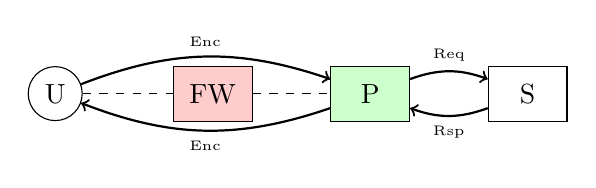
\begin{tikzpicture}[
    scale=0.4,
    node distance=2cm,
    user/.style={circle,draw,minimum size=0.6cm},
    proxy/.style={rectangle,draw,fill=green!20,minimum width=1cm,minimum height=0.7cm},
    server/.style={rectangle,draw,minimum width=1cm,minimum height=0.7cm},
    firewall/.style={rectangle,draw,fill=red!20,minimum width=1cm,minimum height=0.7cm}
]
    % Define nodes
    \node[user] (user) {U};
    \node[firewall] (fw) [right of=user] {FW};
    \node[proxy] (proxy) [right of=fw] {P};
    \node[server] (server) [right of=proxy] {S};

    % Draw arrows and connections
    \draw[->,thick] (user) to[bend left=20] node[above,font=\tiny] {Enc} (proxy);
    \draw[dashed] (user) -- (fw);
    \draw[dashed] (fw) -- (proxy);
    \draw[->,thick] (proxy) to[bend left=20] node[above,font=\tiny] {Req} (server);
    \draw[->,thick] (server) to[bend left=20] node[below,font=\tiny] {Rsp} (proxy);
    \draw[->,thick] (proxy) to[bend left=20] node[below,font=\tiny] {Enc} (user);
\end{tikzpicture}
\end{document}
\caption{Proxy-based network bypass: user (U) connects to server (S) through proxy (P), bypassing firewall restrictions (FW). Encrypted tunnel (Enc) prevents content inspection.}
\label{fig:proxy}
% \vspace{-0.2cm}
\end{figure}

With the evolution of censors, proxy protocols need more sophisticated designs to combat the detection mechanisms that we have mentioned. Whose idea we can conclude as:
\begin{enumerate}
    \item Encryption and Obfuscation
    \item Camouflage
\end{enumerate}

\subsection{Encryption and Obfuscation}
The idea of encryption comes in combat of passive inspections (typically attempt to decrypt), and obfuscation algorithms are additionally designed and put into use in order to reduce distinguishable characteristics of encrypted traffic. 
But as we talked about, unidentifiable encrypted connections (the ideal result of an obfuscation algorithm) can always be suspicious. Furthermore, from the perspective of security, the cipher suites that are adopted by those protocols are not always rigorously verified like mature SSL/TLS stack; from the perspective of engineering, we should better reuse mature solutions rather than reinvent the wheel. 
But those protocols always have a remarkable advantage, they can be stateless can be compatible with UDP forwarding.

\subsubsection{Passive detection}
The mechanism of encryption is just the combination of existing cipher suits, and obfuscation has multiple dimensions:
\begin{itemize}
    \item Manipulating the bytes stream in order to combat byte sequence analysis.
    \item Insert padding bytes in the stream in order to combat packet length analysis.
    \item Alternating the order of sending packets in order to combat timing analysis.
\end{itemize}

\subsubsection{Active probe}
Target to those kinds of proxy servers, the active probe always evaluates servers' reactions and behaviors as we formerly mentioned.

\subsection{Camouflage (Especially as HTTPS Traffic)}
We discussed the advantages which TLS protocol stack can provide seamlessly; in this section, we focus on the mitigations that combat detection approaches. We discuss it with the example of Naiveproxy, one of the best practices of this idea in two perspectives, active probing and passive detection

\subsubsection{Passive detection}
\begin{itemize}
    \item In order to mitigate \textbf{TLS fingerprinting}, Naiveproxy utilizes the network stack of chromium, which is open source and widely adopted. 
    \item \textbf{Packet Length Analysis} can be combated by padding and dividing packets.
    \item  With the utilization of Chromium's network stack, Naiveproxy is supposed not to expose any outstanding \textbf{behaviors} that differ from standard behaviors of Chromium.
\end{itemize}

In practice, we should notice that not only web browsers and Webviews have their own HTTPS implementations; some clients or libraries such as libcURL and OkHTTP also implement HTTPS methods based on TCP, so a client cannot be identified as a web browser does not mean that it is a TLS-based proxy client which tries to camouflage HTTPS connections.


\subsubsection{Active probe}\label{sec:apc}
After the active probing mechanism was revealed, most HTTPS-based protocols adopted combat which is called "Fallback". A valid packet that is initiated by the proxy client should have a proxy header carried credential for authentication. Of course, it is encrypted and embedded in TLS payload. When the authentication fails, it is regarded as a malicious probe. Then the proxy server forwards it to a HTTP server behind. Such a HTTP can both forward it like a mirror station or serve  HTTP content. That will make the proxy server become stealthy to censor and act like a normal website or a mirror site.

\begin{figure}[!h]
    \centering
     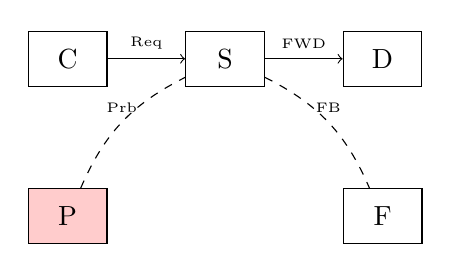
\begin{tikzpicture}[
    scale=0.4, % Further reduced scale
    node distance=2cm, % Further reduced distance
    % user/.style={circle,draw,minimum size=0.6cm},
    % attacker/.style={rectangle,draw,fill=red!20,minimum width=1cm,minimum height=0.7cm},
    % server/.style={rectangle,draw,minimum width=1cm,minimum height=0.7cm}
    censor/.style={rectangle,draw,fill=red!20,minimum width=1cm,minimum height=0.7cm},
    proxy/.style={rectangle,draw,minimum width=1cm,minimum height=0.7cm},
    client/.style={rectangle,draw,minimum width=1cm,minimum height=0.7cm},
    destination/.style={rectangle,draw,minimum width=1cm,minimum height=0.7cm},
    webserver/.style={rectangle,draw,minimum width=1cm,minimum height=0.7cm}
]
    % Define nodes with shorter labels
    % \node[user] (alice) {A};
    % \node[attacker] (mitm) [right of=alice] {M};
    % \node[server] (server) [right of=mitm] {S};
    \node[client] (client) {C};
    \node[censor] (censor) [below of=client] {P};
    \node[proxy] (proxy) [right of=client] {S};
    \node[destination] (destination) [right of=proxy] {D};
    \node[webserver] (webserver) [below of=destination] {F};

    % Shorter arrows and smaller labels
    % \draw[->,thick] (alice) to[bend left=20] node[above,font=\tiny] {Msg} (mitm);
    % \draw[->,thick] (mitm) to[bend left=20] node[above,font=\tiny] {Mod} (server);
    % \draw[->,thick] (server) to[bend left=20] node[below,font=\tiny] {Rsp} (mitm);
    % \draw[->,thick] (mitm) to[bend left=20] node[below,font=\tiny] {Mod} (alice);
    \draw[->] (client) to node[above, font=\tiny] {Req} (proxy);
    \draw[dashed] (censor) to[bend left=20] node[above, font=\tiny] {Prb} (proxy);
    \draw[->] (proxy) to node[above, font=\tiny] {FWD} (destination);
    \draw[dashed] (proxy) to[bend left=20] node[above, font=\tiny] {FB} (webserver);
\end{tikzpicture}
    \caption{Fallback: Proxy servers filter (P) unauthentic incoming traffic (P) (Probes) and forward it to a real HTTP Server (F) and forward authentic traffic (C) to destination (D)}
    \label{fig:fallback}
\end{figure}

\subsection{Conclusion}
In conclusion, the central of network censorship circumvention is camouflage or \textbf{collateral freedom}. In practice, both sides, efforts of detection and circumvention use a combination of those techniques. For example, a protocol based on TLS should also consider its packet length characteristics. There are still some topics and remarkable technologies I cannot cover, such as identifying protocols with Deep Packet Inspection (DPI) in multiple OSI Layers and machine learning. I thought domain fronting used to be an outstanding idea which is one of the best practices of the idea. 
TOR provided domain fronting \cite{domainfronting} based meek bridge \cite{meek} before. Due to various factors such as this technology can also be abused to perform stealthy internet attacks, most CDN providers stopped the support. It also exhibits some temporal characteristics. Internet freedom is a significant topic, and though we focus on the technical details in this paper, we should recognize that it needs a collective effort to defend freedom, as it is a citizen's right that cannot be deprived.

\bibliographystyle{ieeetr}

\bibliography{ref}

\appendix
\section{Setting Up Proxy Server}
In this appendix, we will elaborate on some technical details about our methodology.

\subsection{Software installation}
To set up a remote proxy server, we need to log in the remote server through SSH and pull corresponding software from their official code repository since that software may not be available in the official package registries of most of the Linux distributions, we might be not able to manage in with package manager. 

\subsection{Issue a valid SSL certificate}
For HTTPS-based protocols, we also need to obtain a valid SSL certificate issued by CA (We have discussed why we should not use self-signed certificates). It is possible to use a free SSL certificate that lasts 60 days issued by \href{https://letsencrypt.org/}{Let's Encrypt} or buy one from a CA (usually also a domain registrar), which can be valid longer. For a free SSL certificate, we can also use some tools to automate the process of renewal and installation.

\subsection{Configuration}\label{sec:config}
We made the sample configuration files available in folder \texttt{resources/config}. For more details, please refer to those projects' documents and the Linux man page or send an email to me.

\appendix
\section{Data Collection and Analysis}
We have published the support code and put it in folder \texttt{resources/Code} at the same project. The manual can also be found in \texttt{resources/Manual}.

\end{document}
